\documentclass[1p]{elsarticle_modified}
%\bibliographystyle{elsarticle-num}

%\usepackage[colorlinks]{hyperref}
%\usepackage{abbrmath_seonhwa} %\Abb, \Ascr, \Acal ,\Abf, \Afrak
\usepackage{amsfonts}
\usepackage{amssymb}
\usepackage{amsmath}
\usepackage{amsthm}
\usepackage{scalefnt}
\usepackage{amsbsy}
\usepackage{kotex}
\usepackage{caption}
\usepackage{subfig}
\usepackage{color}
\usepackage{graphicx}
\usepackage{xcolor} %% white, black, red, green, blue, cyan, magenta, yellow
\usepackage{float}
\usepackage{setspace}
\usepackage{hyperref}

\usepackage{tikz}
\usetikzlibrary{arrows}

\usepackage{multirow}
\usepackage{array} % fixed length table
\usepackage{hhline}

%%%%%%%%%%%%%%%%%%%%%
\makeatletter
\renewcommand*\env@matrix[1][\arraystretch]{%
	\edef\arraystretch{#1}%
	\hskip -\arraycolsep
	\let\@ifnextchar\new@ifnextchar
	\array{*\c@MaxMatrixCols c}}
\makeatother %https://tex.stackexchange.com/questions/14071/how-can-i-increase-the-line-spacing-in-a-matrix
%%%%%%%%%%%%%%%

\usepackage[normalem]{ulem}

\newcommand{\msout}[1]{\ifmmode\text{\sout{\ensuremath{#1}}}\else\sout{#1}\fi}
%SOURCE: \msout is \stkout macro in https://tex.stackexchange.com/questions/20609/strikeout-in-math-mode

\newcommand{\cancel}[1]{
	\ifmmode
	{\color{red}\msout{#1}}
	\else
	{\color{red}\sout{#1}}
	\fi
}

\newcommand{\add}[1]{
	{\color{blue}\uwave{#1}}
}

\newcommand{\replace}[2]{
	\ifmmode
	{\color{red}\msout{#1}}{\color{blue}\uwave{#2}}
	\else
	{\color{red}\sout{#1}}{\color{blue}\uwave{#2}}
	\fi
}

\newcommand{\Sol}{\mathcal{S}} %segment
\newcommand{\D}{D} %diagram
\newcommand{\A}{\mathcal{A}} %arc


%%%%%%%%%%%%%%%%%%%%%%%%%%%%%5 test

\def\sl{\operatorname{\textup{SL}}(2,\Cbb)}
\def\psl{\operatorname{\textup{PSL}}(2,\Cbb)}
\def\quan{\mkern 1mu \triangleright \mkern 1mu}

\theoremstyle{definition}
\newtheorem{thm}{Theorem}[section]
\newtheorem{prop}[thm]{Proposition}
\newtheorem{lem}[thm]{Lemma}
\newtheorem{ques}[thm]{Question}
\newtheorem{cor}[thm]{Corollary}
\newtheorem{defn}[thm]{Definition}
\newtheorem{exam}[thm]{Example}
\newtheorem{rmk}[thm]{Remark}
\newtheorem{alg}[thm]{Algorithm}

\newcommand{\I}{\sqrt{-1}}
\begin{document}

%\begin{frontmatter}
%
%\title{Boundary parabolic representations of knots up to 8 crossings}
%
%%% Group authors per affiliation:
%\author{Yunhi Cho} 
%\address{Department of Mathematics, University of Seoul, Seoul, Korea}
%\ead{yhcho@uos.ac.kr}
%
%
%\author{Seonhwa Kim} %\fnref{s_kim}}
%\address{Center for Geometry and Physics, Institute for Basic Science, Pohang, 37673, Korea}
%\ead{ryeona17@ibs.re.kr}
%
%\author{Hyuk Kim}
%\address{Department of Mathematical Sciences, Seoul National University, Seoul 08826, Korea}
%\ead{hyukkim@snu.ac.kr}
%
%\author{Seokbeom Yoon}
%\address{Department of Mathematical Sciences, Seoul National University, Seoul, 08826,  Korea}
%\ead{sbyoon15@snu.ac.kr}
%
%\begin{abstract}
%We find all boundary parabolic representation of knots up to 8 crossings.
%
%\end{abstract}
%\begin{keyword}
%    \MSC[2010] 57M25 
%\end{keyword}
%
%\end{frontmatter}

%\linenumbers
%\tableofcontents
%
\newcommand\colored[1]{\textcolor{white}{\rule[-0.35ex]{0.8em}{1.4ex}}\kern-0.8em\color{red} #1}%
%\newcommand\colored[1]{\textcolor{white}{ #1}\kern-2.17ex	\textcolor{white}{ #1}\kern-1.81ex	\textcolor{white}{ #1}\kern-2.15ex\color{red}#1	}

{\Large $\underline{12a_{0343}~(K12a_{0343})}$}

\setlength{\tabcolsep}{10pt}
\renewcommand{\arraystretch}{1.6}
\vspace{1cm}\begin{tabular}{m{100pt}>{\centering\arraybackslash}m{274pt}}
\multirow{5}{120pt}{
	\centering
	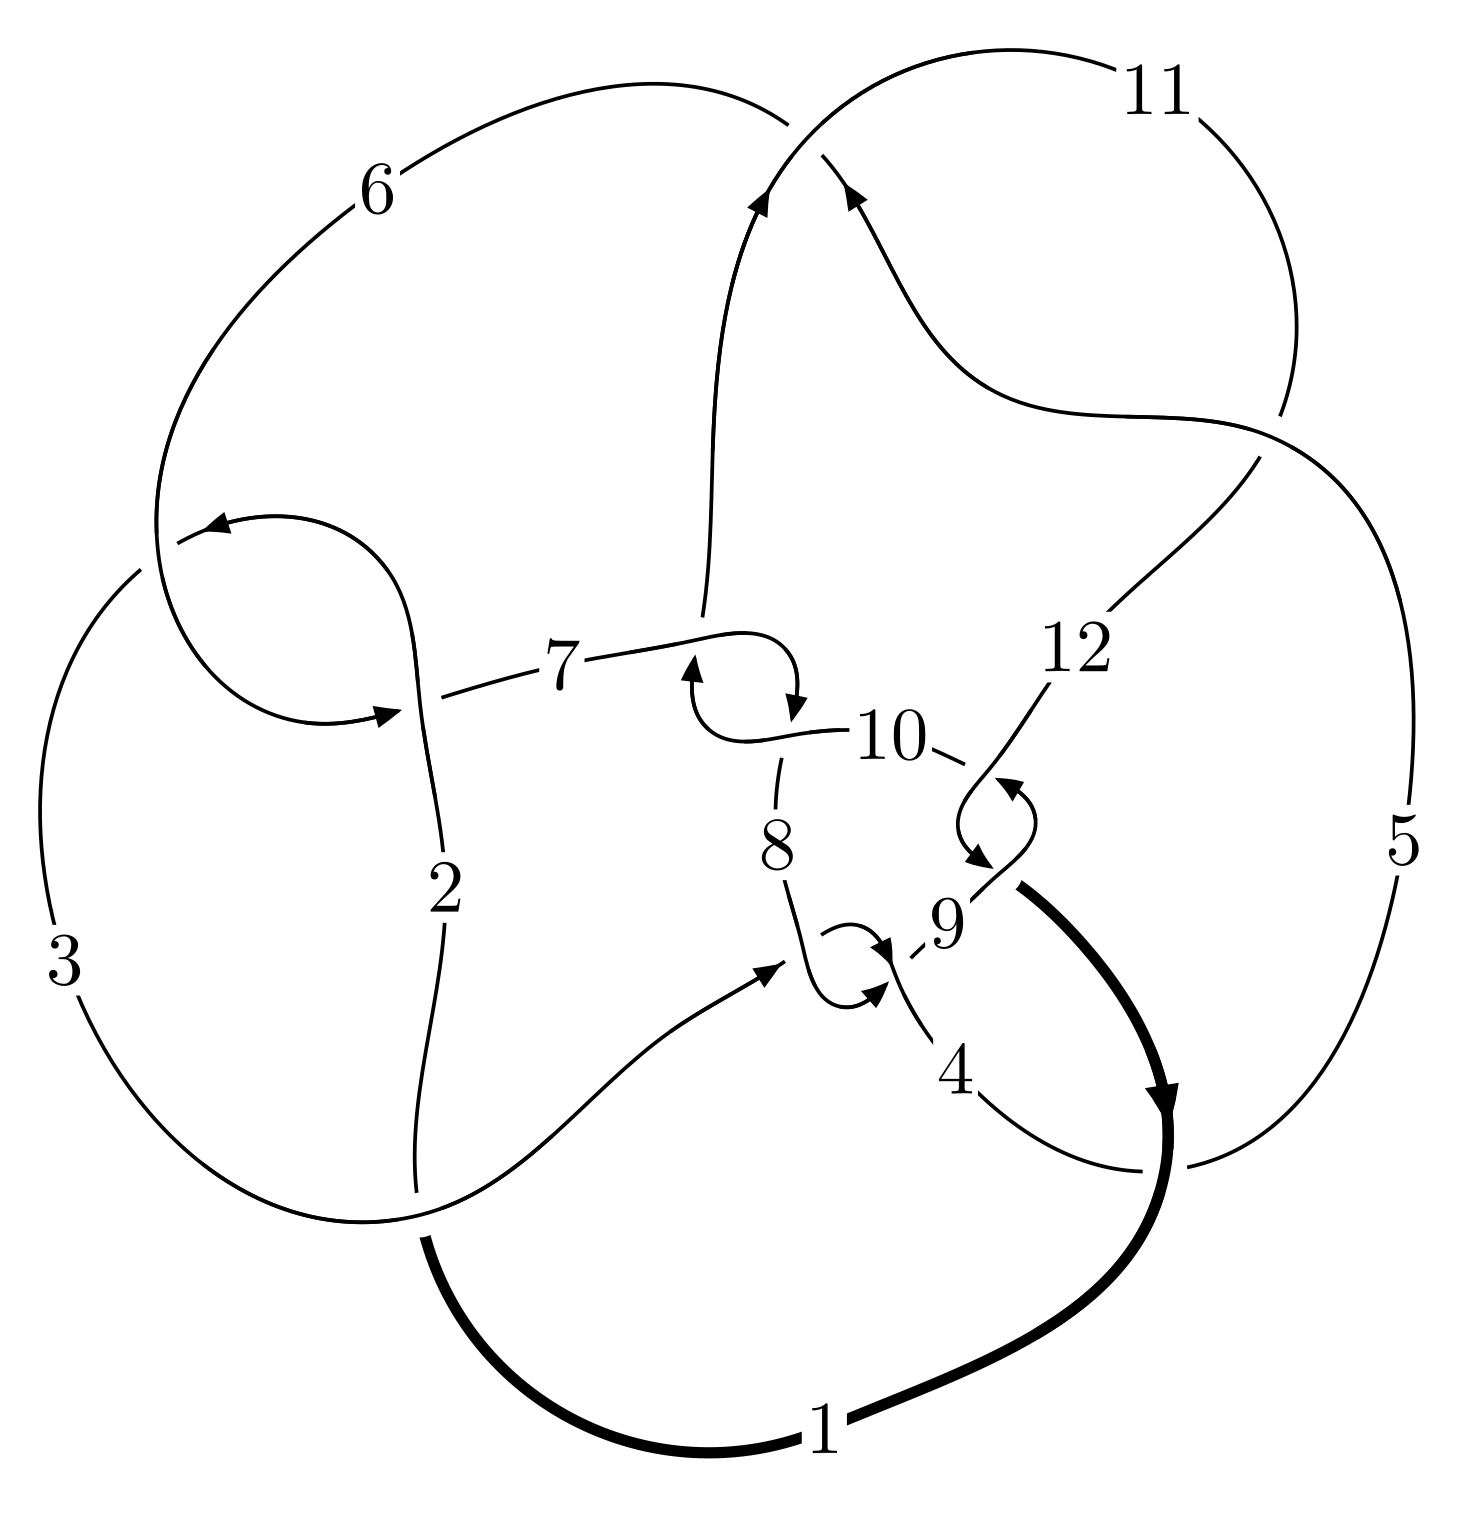
\includegraphics[width=112pt]{../../../GIT/diagram.site/Diagrams/png/1144_12a_0343.png}\\
\ \ \ A knot diagram\footnotemark}&
\allowdisplaybreaks
\textbf{Linearized knot diagam} \\
\cline{2-2}
 &
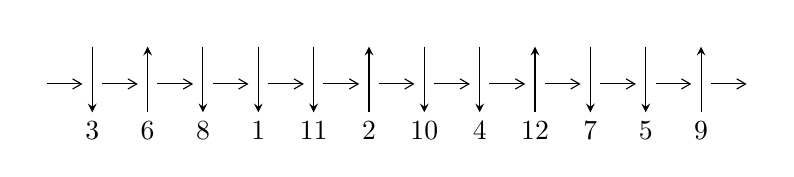
\begin{tikzpicture}[x=20pt, y=17pt]
	% nodes
	\node (C0) at (0, 0) {};
	\node (C1) at (1, 0) {};
	\node (C1U) at (1, +1) {};
	\node (C1D) at (1, -1) {3};

	\node (C2) at (2, 0) {};
	\node (C2U) at (2, +1) {};
	\node (C2D) at (2, -1) {6};

	\node (C3) at (3, 0) {};
	\node (C3U) at (3, +1) {};
	\node (C3D) at (3, -1) {8};

	\node (C4) at (4, 0) {};
	\node (C4U) at (4, +1) {};
	\node (C4D) at (4, -1) {1};

	\node (C5) at (5, 0) {};
	\node (C5U) at (5, +1) {};
	\node (C5D) at (5, -1) {11};

	\node (C6) at (6, 0) {};
	\node (C6U) at (6, +1) {};
	\node (C6D) at (6, -1) {2};

	\node (C7) at (7, 0) {};
	\node (C7U) at (7, +1) {};
	\node (C7D) at (7, -1) {10};

	\node (C8) at (8, 0) {};
	\node (C8U) at (8, +1) {};
	\node (C8D) at (8, -1) {4};

	\node (C9) at (9, 0) {};
	\node (C9U) at (9, +1) {};
	\node (C9D) at (9, -1) {12};

	\node (C10) at (10, 0) {};
	\node (C10U) at (10, +1) {};
	\node (C10D) at (10, -1) {7};

	\node (C11) at (11, 0) {};
	\node (C11U) at (11, +1) {};
	\node (C11D) at (11, -1) {5};

	\node (C12) at (12, 0) {};
	\node (C12U) at (12, +1) {};
	\node (C12D) at (12, -1) {9};
	\node (C13) at (13, 0) {};

	% arrows
	\draw[->,>={angle 60}]
	(C0) edge (C1) (C1) edge (C2) (C2) edge (C3) (C3) edge (C4) (C4) edge (C5) (C5) edge (C6) (C6) edge (C7) (C7) edge (C8) (C8) edge (C9) (C9) edge (C10) (C10) edge (C11) (C11) edge (C12) (C12) edge (C13) ;	\draw[->,>=stealth]
	(C1U) edge (C1D) (C2D) edge (C2U) (C3U) edge (C3D) (C4U) edge (C4D) (C5U) edge (C5D) (C6D) edge (C6U) (C7U) edge (C7D) (C8U) edge (C8D) (C9D) edge (C9U) (C10U) edge (C10D) (C11U) edge (C11D) (C12D) edge (C12U) ;
	\end{tikzpicture} \\
\hhline{~~} \\& 
\textbf{Solving Sequence} \\ \cline{2-2} 
 &
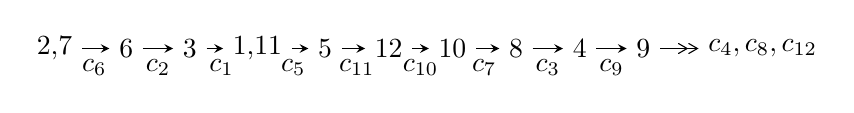
\begin{tikzpicture}[x=23pt, y=7pt]
	% node
	\node (A0) at (-1/8, 0) {2,7};
	\node (A1) at (1, 0) {6};
	\node (A2) at (2, 0) {3};
	\node (A3) at (49/16, 0) {1,11};
	\node (A4) at (33/8, 0) {5};
	\node (A5) at (41/8, 0) {12};
	\node (A6) at (49/8, 0) {10};
	\node (A7) at (57/8, 0) {8};
	\node (A8) at (65/8, 0) {4};
	\node (A9) at (73/8, 0) {9};
	\node (C1) at (1/2, -1) {$c_{6}$};
	\node (C2) at (3/2, -1) {$c_{2}$};
	\node (C3) at (5/2, -1) {$c_{1}$};
	\node (C4) at (29/8, -1) {$c_{5}$};
	\node (C5) at (37/8, -1) {$c_{11}$};
	\node (C6) at (45/8, -1) {$c_{10}$};
	\node (C7) at (53/8, -1) {$c_{7}$};
	\node (C8) at (61/8, -1) {$c_{3}$};
	\node (C9) at (69/8, -1) {$c_{9}$};
	\node (A10) at (11, 0) {$c_{4},c_{8},c_{12}$};

	% edge
	\draw[->,>=stealth]	
	(A0) edge (A1) (A1) edge (A2) (A2) edge (A3) (A3) edge (A4) (A4) edge (A5) (A5) edge (A6) (A6) edge (A7) (A7) edge (A8) (A8) edge (A9) ;
	\draw[->>,>={angle 60}]	
	(A9) edge (A10);
\end{tikzpicture} \\ 

\end{tabular} \\

\footnotetext{
The image of knot diagram is generated by the software ``\textbf{Draw programme}" developed by Andrew Bartholomew(\url{http://www.layer8.co.uk/maths/draw/index.htm\#Running-draw}), where we modified some parts for our purpose(\url{https://github.com/CATsTAILs/LinksPainter}).
}\phantom \\ \newline 
\centering \textbf{Ideals for irreducible components\footnotemark of $X_{\text{par}}$} 
 
\begin{align*}
I^u_{1}&=\langle 
-1.89950\times10^{307} u^{122}-3.45185\times10^{305} u^{121}+\cdots+2.69069\times10^{307} b-8.18602\times10^{307},\\
\phantom{I^u_{1}}&\phantom{= \langle  }8.09068\times10^{306} u^{122}-2.25508\times10^{306} u^{121}+\cdots+2.69069\times10^{307} a+3.45678\times10^{308},\;u^{123}- u^{122}+\cdots-20 u+1\rangle \\
I^u_{2}&=\langle 
-39 u^{23}-150 u^{22}+\cdots+11 b+5,\;56 u^{23}+267 u^{22}+\cdots+11 a+144,\;u^{24}+4 u^{23}+\cdots+4 u+1\rangle \\
\\
\end{align*}
\raggedright * 2 irreducible components of $\dim_{\mathbb{C}}=0$, with total 147 representations.\\
\footnotetext{All coefficients of polynomials are rational numbers. But the coefficients are sometimes approximated in decimal forms when there is not enough margin.}
\newpage
\renewcommand{\arraystretch}{1}
\centering \section*{I. $I^u_{1}= \langle -1.90\times10^{307} u^{122}-3.45\times10^{305} u^{121}+\cdots+2.69\times10^{307} b-8.19\times10^{307},\;8.09\times10^{306} u^{122}-2.26\times10^{306} u^{121}+\cdots+2.69\times10^{307} a+3.46\times10^{308},\;u^{123}- u^{122}+\cdots-20 u+1 \rangle$}
\flushleft \textbf{(i) Arc colorings}\\
\begin{tabular}{m{7pt} m{180pt} m{7pt} m{180pt} }
\flushright $a_{2}=$&$\begin{pmatrix}0\\u\end{pmatrix}$ \\
\flushright $a_{7}=$&$\begin{pmatrix}1\\0\end{pmatrix}$ \\
\flushright $a_{6}=$&$\begin{pmatrix}1\\u^2\end{pmatrix}$ \\
\flushright $a_{3}=$&$\begin{pmatrix}u\\u^3+u\end{pmatrix}$ \\
\flushright $a_{1}=$&$\begin{pmatrix}u^3\\u^5+u^3+u\end{pmatrix}$ \\
\flushright $a_{11}=$&$\begin{pmatrix}-0.300691 u^{122}+0.0838104 u^{121}+\cdots+142.979 u-12.8472\\0.705952 u^{122}+0.0128289 u^{121}+\cdots-44.7302 u+3.04235\end{pmatrix}$ \\
\flushright $a_{5}=$&$\begin{pmatrix}6.23437 u^{122}-3.57871 u^{121}+\cdots+597.596 u-37.9819\\-0.328481 u^{122}+0.685943 u^{121}+\cdots-0.169787 u-0.237379\end{pmatrix}$ \\
\flushright $a_{12}=$&$\begin{pmatrix}-9.17317 u^{122}+3.03651 u^{121}+\cdots+237.883 u-14.9968\\-2.75634 u^{122}+1.33344 u^{121}+\cdots-51.5139 u+2.67282\end{pmatrix}$ \\
\flushright $a_{10}=$&$\begin{pmatrix}0.405261 u^{122}+0.0966392 u^{121}+\cdots+98.2485 u-9.80483\\0.705952 u^{122}+0.0128289 u^{121}+\cdots-44.7302 u+3.04235\end{pmatrix}$ \\
\flushright $a_{8}=$&$\begin{pmatrix}-2.82246 u^{122}+3.05333 u^{121}+\cdots-473.089 u+33.5336\\1.04326 u^{122}-0.380472 u^{121}+\cdots-4.60280 u+0.669294\end{pmatrix}$ \\
\flushright $a_{4}=$&$\begin{pmatrix}5.75868 u^{122}-3.43889 u^{121}+\cdots+592.906 u-37.7562\\-0.598238 u^{122}+0.690271 u^{121}+\cdots-5.88629 u+0.266081\end{pmatrix}$ \\
\flushright $a_{9}=$&$\begin{pmatrix}1.80034 u^{122}+4.11751 u^{121}+\cdots+68.8102 u+2.53731\\0.0935492 u^{122}+1.97398 u^{121}+\cdots-53.4074 u+3.58507\end{pmatrix}$\\&\end{tabular}
\flushleft \textbf{(ii) Obstruction class $= -1$}\\~\\
\flushleft \textbf{(iii) Cusp Shapes $= -12.1423 u^{122}+7.17995 u^{121}+\cdots-672.463 u+44.2835$}\\~\\
\newpage\renewcommand{\arraystretch}{1}
\flushleft \textbf{(iv) u-Polynomials at the component}\newline \\
\begin{tabular}{m{50pt}|m{274pt}}
Crossings & \hspace{64pt}u-Polynomials at each crossing \\
\hline $$\begin{aligned}c_{1}\end{aligned}$$&$\begin{aligned}
&u^{123}+47 u^{122}+\cdots-78 u-1
\end{aligned}$\\
\hline $$\begin{aligned}c_{2},c_{6}\end{aligned}$$&$\begin{aligned}
&u^{123}- u^{122}+\cdots-20 u+1
\end{aligned}$\\
\hline $$\begin{aligned}c_{3},c_{8}\end{aligned}$$&$\begin{aligned}
&u^{123}- u^{122}+\cdots-96274 u+98677
\end{aligned}$\\
\hline $$\begin{aligned}c_{4}\end{aligned}$$&$\begin{aligned}
&u^{123}-3 u^{122}+\cdots-639124 u+39811
\end{aligned}$\\
\hline $$\begin{aligned}c_{5},c_{11}\end{aligned}$$&$\begin{aligned}
&u^{123}+5 u^{122}+\cdots+1222892 u+197593
\end{aligned}$\\
\hline $$\begin{aligned}c_{7},c_{10}\end{aligned}$$&$\begin{aligned}
&u^{123}-5 u^{122}+\cdots-16144 u+3433
\end{aligned}$\\
\hline $$\begin{aligned}c_{9},c_{12}\end{aligned}$$&$\begin{aligned}
&u^{123}+5 u^{122}+\cdots-10837 u+889
\end{aligned}$\\
\hline
\end{tabular}\\~\\
\newpage\renewcommand{\arraystretch}{1}
\flushleft \textbf{(v) Riley Polynomials at the component}\newline \\
\begin{tabular}{m{50pt}|m{274pt}}
Crossings & \hspace{64pt}Riley Polynomials at each crossing \\
\hline $$\begin{aligned}c_{1}\end{aligned}$$&$\begin{aligned}
&y^{123}+67 y^{122}+\cdots+7218 y-1
\end{aligned}$\\
\hline $$\begin{aligned}c_{2},c_{6}\end{aligned}$$&$\begin{aligned}
&y^{123}+47 y^{122}+\cdots-78 y-1
\end{aligned}$\\
\hline $$\begin{aligned}c_{3},c_{8}\end{aligned}$$&$\begin{aligned}
&y^{123}-79 y^{122}+\cdots+21540154796 y-9737150329
\end{aligned}$\\
\hline $$\begin{aligned}c_{4}\end{aligned}$$&$\begin{aligned}
&y^{123}-23 y^{122}+\cdots+63443203538 y-1584915721
\end{aligned}$\\
\hline $$\begin{aligned}c_{5},c_{11}\end{aligned}$$&$\begin{aligned}
&y^{123}+91 y^{122}+\cdots-210187966472 y-39042993649
\end{aligned}$\\
\hline $$\begin{aligned}c_{7},c_{10}\end{aligned}$$&$\begin{aligned}
&y^{123}+91 y^{122}+\cdots-3783445264 y-11785489
\end{aligned}$\\
\hline $$\begin{aligned}c_{9},c_{12}\end{aligned}$$&$\begin{aligned}
&y^{123}+81 y^{122}+\cdots-9554859 y-790321
\end{aligned}$\\
\hline
\end{tabular}\\~\\
\newpage\flushleft \textbf{(vi) Complex Volumes and Cusp Shapes}
$$\begin{array}{c|c|c}  
\text{Solutions to }I^u_{1}& \I (\text{vol} + \sqrt{-1}CS) & \text{Cusp shape}\\
 \hline 
\begin{aligned}
u &= \phantom{-}0.548242 + 0.829520 I \\
a &= -0.28443 + 3.46875 I \\
b &= \phantom{-}0.010383 + 1.086070 I\end{aligned}
 & \phantom{-}0.28408 + 1.97118 I & \phantom{-0.000000 } 0 \\ \hline\begin{aligned}
u &= \phantom{-}0.548242 - 0.829520 I \\
a &= -0.28443 - 3.46875 I \\
b &= \phantom{-}0.010383 - 1.086070 I\end{aligned}
 & \phantom{-}0.28408 - 1.97118 I & \phantom{-0.000000 } 0 \\ \hline\begin{aligned}
u &= \phantom{-}0.188873 + 0.961874 I \\
a &= \phantom{-}1.06444 - 1.90209 I \\
b &= -0.487294 + 0.744193 I\end{aligned}
 & -1.65857 + 2.76829 I & \phantom{-0.000000 } 0 \\ \hline\begin{aligned}
u &= \phantom{-}0.188873 - 0.961874 I \\
a &= \phantom{-}1.06444 + 1.90209 I \\
b &= -0.487294 - 0.744193 I\end{aligned}
 & -1.65857 - 2.76829 I & \phantom{-0.000000 } 0 \\ \hline\begin{aligned}
u &= \phantom{-}0.471154 + 0.913310 I \\
a &= \phantom{-}0.207239 - 1.003520 I \\
b &= \phantom{-}0.0108251 + 0.0804532 I\end{aligned}
 & -1.62654 + 2.08087 I & \phantom{-0.000000 } 0 \\ \hline\begin{aligned}
u &= \phantom{-}0.471154 - 0.913310 I \\
a &= \phantom{-}0.207239 + 1.003520 I \\
b &= \phantom{-}0.0108251 - 0.0804532 I\end{aligned}
 & -1.62654 - 2.08087 I & \phantom{-0.000000 } 0 \\ \hline\begin{aligned}
u &= \phantom{-}0.663578 + 0.788429 I \\
a &= -0.737189 - 0.836372 I \\
b &= \phantom{-}0.217628 - 1.232180 I\end{aligned}
 & \phantom{-}2.85574 + 2.86066 I & \phantom{-0.000000 } 0 \\ \hline\begin{aligned}
u &= \phantom{-}0.663578 - 0.788429 I \\
a &= -0.737189 + 0.836372 I \\
b &= \phantom{-}0.217628 + 1.232180 I\end{aligned}
 & \phantom{-}2.85574 - 2.86066 I & \phantom{-0.000000 } 0 \\ \hline\begin{aligned}
u &= \phantom{-}0.692386 + 0.663598 I \\
a &= \phantom{-}1.04127 + 1.31583 I \\
b &= -1.403510 - 0.137517 I\end{aligned}
 & -2.19824 - 6.06325 I & \phantom{-0.000000 } 0 \\ \hline\begin{aligned}
u &= \phantom{-}0.692386 - 0.663598 I \\
a &= \phantom{-}1.04127 - 1.31583 I \\
b &= -1.403510 + 0.137517 I\end{aligned}
 & -2.19824 + 6.06325 I & \phantom{-0.000000 } 0\\
 \hline 
 \end{array}$$\newpage$$\begin{array}{c|c|c}  
\text{Solutions to }I^u_{1}& \I (\text{vol} + \sqrt{-1}CS) & \text{Cusp shape}\\
 \hline 
\begin{aligned}
u &= -0.684030 + 0.787122 I \\
a &= -0.718927 + 0.734117 I \\
b &= \phantom{-}1.090480 - 0.430052 I\end{aligned}
 & \phantom{-}1.08865 + 1.42170 I & \phantom{-0.000000 } 0 \\ \hline\begin{aligned}
u &= -0.684030 - 0.787122 I \\
a &= -0.718927 - 0.734117 I \\
b &= \phantom{-}1.090480 + 0.430052 I\end{aligned}
 & \phantom{-}1.08865 - 1.42170 I & \phantom{-0.000000 } 0 \\ \hline\begin{aligned}
u &= -0.867245 + 0.598841 I \\
a &= -0.117871 - 0.088053 I \\
b &= \phantom{-}0.37530 - 1.45134 I\end{aligned}
 & \phantom{-}7.05300 + 6.39208 I & \phantom{-0.000000 } 0 \\ \hline\begin{aligned}
u &= -0.867245 - 0.598841 I \\
a &= -0.117871 + 0.088053 I \\
b &= \phantom{-}0.37530 + 1.45134 I\end{aligned}
 & \phantom{-}7.05300 - 6.39208 I & \phantom{-0.000000 } 0 \\ \hline\begin{aligned}
u &= \phantom{-}0.054989 + 1.056020 I \\
a &= \phantom{-}1.33622 + 0.58354 I \\
b &= -0.884436 + 0.596936 I\end{aligned}
 & -6.96479 - 5.41961 I & \phantom{-0.000000 } 0 \\ \hline\begin{aligned}
u &= \phantom{-}0.054989 - 1.056020 I \\
a &= \phantom{-}1.33622 - 0.58354 I \\
b &= -0.884436 - 0.596936 I\end{aligned}
 & -6.96479 + 5.41961 I & \phantom{-0.000000 } 0 \\ \hline\begin{aligned}
u &= -0.777613 + 0.728742 I \\
a &= \phantom{-}0.446166 + 0.395572 I \\
b &= \phantom{-}0.59916 - 1.66153 I\end{aligned}
 & \phantom{-}4.59202 + 0.63566 I & \phantom{-0.000000 } 0 \\ \hline\begin{aligned}
u &= -0.777613 - 0.728742 I \\
a &= \phantom{-}0.446166 - 0.395572 I \\
b &= \phantom{-}0.59916 + 1.66153 I\end{aligned}
 & \phantom{-}4.59202 - 0.63566 I & \phantom{-0.000000 } 0 \\ \hline\begin{aligned}
u &= \phantom{-}0.555401 + 0.915721 I \\
a &= -3.63550 - 0.10365 I \\
b &= \phantom{-}0.119236 - 0.990652 I\end{aligned}
 & -0.01039 + 2.42514 I & \phantom{-0.000000 } 0 \\ \hline\begin{aligned}
u &= \phantom{-}0.555401 - 0.915721 I \\
a &= -3.63550 + 0.10365 I \\
b &= \phantom{-}0.119236 + 0.990652 I\end{aligned}
 & -0.01039 - 2.42514 I & \phantom{-0.000000 } 0\\
 \hline 
 \end{array}$$\newpage$$\begin{array}{c|c|c}  
\text{Solutions to }I^u_{1}& \I (\text{vol} + \sqrt{-1}CS) & \text{Cusp shape}\\
 \hline 
\begin{aligned}
u &= -0.701386 + 0.596129 I \\
a &= -0.610071 + 1.182720 I \\
b &= -0.311639 + 1.042460 I\end{aligned}
 & -2.82441 + 6.67098 I & \phantom{-0.000000 } 0 \\ \hline\begin{aligned}
u &= -0.701386 - 0.596129 I \\
a &= -0.610071 - 1.182720 I \\
b &= -0.311639 - 1.042460 I\end{aligned}
 & -2.82441 - 6.67098 I & \phantom{-0.000000 } 0 \\ \hline\begin{aligned}
u &= \phantom{-}0.564981 + 0.726132 I \\
a &= \phantom{-}0.267380 - 0.658452 I \\
b &= \phantom{-}0.61470 + 1.80552 I\end{aligned}
 & \phantom{-}4.79658 - 1.21676 I & \phantom{-0.000000 } 0 \\ \hline\begin{aligned}
u &= \phantom{-}0.564981 - 0.726132 I \\
a &= \phantom{-}0.267380 + 0.658452 I \\
b &= \phantom{-}0.61470 - 1.80552 I\end{aligned}
 & \phantom{-}4.79658 + 1.21676 I & \phantom{-0.000000 } 0 \\ \hline\begin{aligned}
u &= \phantom{-}0.092365 + 0.914757 I \\
a &= -1.79744 + 0.67550 I \\
b &= \phantom{-}0.701179 - 0.034836 I\end{aligned}
 & -3.74968 + 2.54946 I & \phantom{-0.000000 } 0 \\ \hline\begin{aligned}
u &= \phantom{-}0.092365 - 0.914757 I \\
a &= -1.79744 - 0.67550 I \\
b &= \phantom{-}0.701179 + 0.034836 I\end{aligned}
 & -3.74968 - 2.54946 I & \phantom{-0.000000 } 0 \\ \hline\begin{aligned}
u &= -0.795084 + 0.738844 I \\
a &= -0.117741 - 0.649836 I \\
b &= -0.94381 + 1.52052 I\end{aligned}
 & \phantom{-}4.61157 + 1.84512 I & \phantom{-0.000000 } 0 \\ \hline\begin{aligned}
u &= -0.795084 - 0.738844 I \\
a &= -0.117741 + 0.649836 I \\
b &= -0.94381 - 1.52052 I\end{aligned}
 & \phantom{-}4.61157 - 1.84512 I & \phantom{-0.000000 } 0 \\ \hline\begin{aligned}
u &= \phantom{-}0.571873 + 0.702674 I \\
a &= -0.673278 - 0.065065 I \\
b &= -0.01582 - 1.84927 I\end{aligned}
 & \phantom{-}4.72306 + 3.41874 I & \phantom{-0.000000 } 0 \\ \hline\begin{aligned}
u &= \phantom{-}0.571873 - 0.702674 I \\
a &= -0.673278 + 0.065065 I \\
b &= -0.01582 + 1.84927 I\end{aligned}
 & \phantom{-}4.72306 - 3.41874 I & \phantom{-0.000000 } 0\\
 \hline 
 \end{array}$$\newpage$$\begin{array}{c|c|c}  
\text{Solutions to }I^u_{1}& \I (\text{vol} + \sqrt{-1}CS) & \text{Cusp shape}\\
 \hline 
\begin{aligned}
u &= -0.044210 + 1.100950 I \\
a &= \phantom{-}1.28678 - 0.62406 I \\
b &= -0.720657 + 0.969939 I\end{aligned}
 & -7.91882 + 5.51597 I & \phantom{-0.000000 } 0 \\ \hline\begin{aligned}
u &= -0.044210 - 1.100950 I \\
a &= \phantom{-}1.28678 + 0.62406 I \\
b &= -0.720657 - 0.969939 I\end{aligned}
 & -7.91882 - 5.51597 I & \phantom{-0.000000 } 0 \\ \hline\begin{aligned}
u &= -0.668230 + 0.600020 I \\
a &= \phantom{-}0.965540 - 0.874576 I \\
b &= \phantom{-}0.072062 - 1.171120 I\end{aligned}
 & \phantom{-}2.09455 + 2.14303 I & \phantom{-0.000000 } 0 \\ \hline\begin{aligned}
u &= -0.668230 - 0.600020 I \\
a &= \phantom{-}0.965540 + 0.874576 I \\
b &= \phantom{-}0.072062 + 1.171120 I\end{aligned}
 & \phantom{-}2.09455 - 2.14303 I & \phantom{-0.000000 } 0 \\ \hline\begin{aligned}
u &= -0.704145 + 0.853571 I \\
a &= \phantom{-}1.059400 - 0.583116 I \\
b &= -0.844367 + 0.144764 I\end{aligned}
 & \phantom{-}4.58356 - 2.69549 I & \phantom{-0.000000 } 0 \\ \hline\begin{aligned}
u &= -0.704145 - 0.853571 I \\
a &= \phantom{-}1.059400 + 0.583116 I \\
b &= -0.844367 - 0.144764 I\end{aligned}
 & \phantom{-}4.58356 + 2.69549 I & \phantom{-0.000000 } 0 \\ \hline\begin{aligned}
u &= \phantom{-}0.657481 + 0.915129 I \\
a &= \phantom{-}1.39700 + 0.30229 I \\
b &= -0.044526 + 1.168290 I\end{aligned}
 & \phantom{-}2.46284 + 2.27208 I & \phantom{-0.000000 } 0 \\ \hline\begin{aligned}
u &= \phantom{-}0.657481 - 0.915129 I \\
a &= \phantom{-}1.39700 - 0.30229 I \\
b &= -0.044526 - 1.168290 I\end{aligned}
 & \phantom{-}2.46284 - 2.27208 I & \phantom{-0.000000 } 0 \\ \hline\begin{aligned}
u &= \phantom{-}0.603634 + 0.625438 I \\
a &= -0.95310 - 1.22694 I \\
b &= \phantom{-}0.917200 + 0.488596 I\end{aligned}
 & \phantom{-}1.61464 - 1.48578 I & \phantom{-0.000000 } 0 \\ \hline\begin{aligned}
u &= \phantom{-}0.603634 - 0.625438 I \\
a &= -0.95310 + 1.22694 I \\
b &= \phantom{-}0.917200 - 0.488596 I\end{aligned}
 & \phantom{-}1.61464 + 1.48578 I & \phantom{-0.000000 } 0\\
 \hline 
 \end{array}$$\newpage$$\begin{array}{c|c|c}  
\text{Solutions to }I^u_{1}& \I (\text{vol} + \sqrt{-1}CS) & \text{Cusp shape}\\
 \hline 
\begin{aligned}
u &= -0.930561 + 0.651530 I \\
a &= \phantom{-}0.0935930 - 0.0169775 I \\
b &= -0.297784 + 1.346470 I\end{aligned}
 & \phantom{-}9.44491 + 1.26369 I & \phantom{-0.000000 } 0 \\ \hline\begin{aligned}
u &= -0.930561 - 0.651530 I \\
a &= \phantom{-}0.0935930 + 0.0169775 I \\
b &= -0.297784 - 1.346470 I\end{aligned}
 & \phantom{-}9.44491 - 1.26369 I & \phantom{-0.000000 } 0 \\ \hline\begin{aligned}
u &= \phantom{-}0.039146 + 0.856732 I \\
a &= -0.28892 + 1.55625 I \\
b &= \phantom{-}0.454781 - 0.796880 I\end{aligned}
 & -0.95020 + 1.54615 I & \phantom{-0.000000 } 0 \\ \hline\begin{aligned}
u &= \phantom{-}0.039146 - 0.856732 I \\
a &= -0.28892 - 1.55625 I \\
b &= \phantom{-}0.454781 + 0.796880 I\end{aligned}
 & -0.95020 - 1.54615 I & \phantom{-0.000000 } 0 \\ \hline\begin{aligned}
u &= -0.690055 + 0.913609 I \\
a &= -1.34483 + 0.79702 I \\
b &= \phantom{-}1.081260 + 0.213210 I\end{aligned}
 & \phantom{-}0.70739 - 6.71925 I & \phantom{-0.000000 } 0 \\ \hline\begin{aligned}
u &= -0.690055 - 0.913609 I \\
a &= -1.34483 - 0.79702 I \\
b &= \phantom{-}1.081260 - 0.213210 I\end{aligned}
 & \phantom{-}0.70739 + 6.71925 I & \phantom{-0.000000 } 0 \\ \hline\begin{aligned}
u &= \phantom{-}0.594792 + 0.982560 I \\
a &= -2.26229 + 0.28907 I \\
b &= \phantom{-}0.79501 - 1.51106 I\end{aligned}
 & \phantom{-}3.93905 + 5.86747 I & \phantom{-0.000000 } 0 \\ \hline\begin{aligned}
u &= \phantom{-}0.594792 - 0.982560 I \\
a &= -2.26229 - 0.28907 I \\
b &= \phantom{-}0.79501 + 1.51106 I\end{aligned}
 & \phantom{-}3.93905 - 5.86747 I & \phantom{-0.000000 } 0 \\ \hline\begin{aligned}
u &= -0.228702 + 1.126900 I \\
a &= \phantom{-}1.50308 + 0.18992 I \\
b &= -0.845488 - 0.603207 I\end{aligned}
 & -8.99015 - 0.16187 I & \phantom{-0.000000 } 0 \\ \hline\begin{aligned}
u &= -0.228702 - 1.126900 I \\
a &= \phantom{-}1.50308 - 0.18992 I \\
b &= -0.845488 + 0.603207 I\end{aligned}
 & -8.99015 + 0.16187 I & \phantom{-0.000000 } 0\\
 \hline 
 \end{array}$$\newpage$$\begin{array}{c|c|c}  
\text{Solutions to }I^u_{1}& \I (\text{vol} + \sqrt{-1}CS) & \text{Cusp shape}\\
 \hline 
\begin{aligned}
u &= \phantom{-}0.075421 + 1.150460 I \\
a &= -0.62923 + 1.66673 I \\
b &= \phantom{-}0.143974 - 1.211900 I\end{aligned}
 & \phantom{-}0.42044 + 5.23178 I & \phantom{-0.000000 } 0 \\ \hline\begin{aligned}
u &= \phantom{-}0.075421 - 1.150460 I \\
a &= -0.62923 - 1.66673 I \\
b &= \phantom{-}0.143974 + 1.211900 I\end{aligned}
 & \phantom{-}0.42044 - 5.23178 I & \phantom{-0.000000 } 0 \\ \hline\begin{aligned}
u &= \phantom{-}0.842806 + 0.801573 I \\
a &= \phantom{-}0.929607 + 0.697534 I \\
b &= -0.578522 + 1.001110 I\end{aligned}
 & -1.36378 + 5.18885 I & \phantom{-0.000000 } 0 \\ \hline\begin{aligned}
u &= \phantom{-}0.842806 - 0.801573 I \\
a &= \phantom{-}0.929607 - 0.697534 I \\
b &= -0.578522 - 1.001110 I\end{aligned}
 & -1.36378 - 5.18885 I & \phantom{-0.000000 } 0 \\ \hline\begin{aligned}
u &= \phantom{-}0.199194 + 1.146730 I \\
a &= \phantom{-}0.53743 - 1.54694 I \\
b &= \phantom{-}0.137196 + 1.073490 I\end{aligned}
 & \phantom{-}1.68007 + 0.55799 I & \phantom{-0.000000 } 0 \\ \hline\begin{aligned}
u &= \phantom{-}0.199194 - 1.146730 I \\
a &= \phantom{-}0.53743 + 1.54694 I \\
b &= \phantom{-}0.137196 - 1.073490 I\end{aligned}
 & \phantom{-}1.68007 - 0.55799 I & \phantom{-0.000000 } 0 \\ \hline\begin{aligned}
u &= \phantom{-}0.790044 + 0.860801 I \\
a &= -0.367226 - 0.181117 I \\
b &= -0.366840 - 0.928566 I\end{aligned}
 & -1.49647 + 0.88140 I & \phantom{-0.000000 } 0 \\ \hline\begin{aligned}
u &= \phantom{-}0.790044 - 0.860801 I \\
a &= -0.367226 + 0.181117 I \\
b &= -0.366840 + 0.928566 I\end{aligned}
 & -1.49647 - 0.88140 I & \phantom{-0.000000 } 0 \\ \hline\begin{aligned}
u &= \phantom{-}1.015760 + 0.586708 I \\
a &= -0.0011892 + 0.0495695 I \\
b &= -0.53755 - 1.44463 I\end{aligned}
 & \phantom{-}2.89061 - 12.49430 I & \phantom{-0.000000 } 0 \\ \hline\begin{aligned}
u &= \phantom{-}1.015760 - 0.586708 I \\
a &= -0.0011892 - 0.0495695 I \\
b &= -0.53755 + 1.44463 I\end{aligned}
 & \phantom{-}2.89061 + 12.49430 I & \phantom{-0.000000 } 0\\
 \hline 
 \end{array}$$\newpage$$\begin{array}{c|c|c}  
\text{Solutions to }I^u_{1}& \I (\text{vol} + \sqrt{-1}CS) & \text{Cusp shape}\\
 \hline 
\begin{aligned}
u &= \phantom{-}0.622172 + 0.996075 I \\
a &= \phantom{-}1.90904 - 0.51865 I \\
b &= -0.29135 + 1.61684 I\end{aligned}
 & \phantom{-}3.74029 + 1.37980 I & \phantom{-0.000000 } 0 \\ \hline\begin{aligned}
u &= \phantom{-}0.622172 - 0.996075 I \\
a &= \phantom{-}1.90904 + 0.51865 I \\
b &= -0.29135 - 1.61684 I\end{aligned}
 & \phantom{-}3.74029 - 1.37980 I & \phantom{-0.000000 } 0 \\ \hline\begin{aligned}
u &= -0.398934 + 1.105590 I \\
a &= -0.943165 + 0.353299 I \\
b &= \phantom{-}0.743394 + 0.242700 I\end{aligned}
 & -4.33976 - 3.64831 I & \phantom{-0.000000 } 0 \\ \hline\begin{aligned}
u &= -0.398934 - 1.105590 I \\
a &= -0.943165 - 0.353299 I \\
b &= \phantom{-}0.743394 - 0.242700 I\end{aligned}
 & -4.33976 + 3.64831 I & \phantom{-0.000000 } 0 \\ \hline\begin{aligned}
u &= \phantom{-}0.292366 + 0.769927 I \\
a &= \phantom{-}0.811956 + 0.272617 I \\
b &= -0.140390 - 0.142748 I\end{aligned}
 & -0.402159 + 1.260340 I & \phantom{-0.000000 } 0 \\ \hline\begin{aligned}
u &= \phantom{-}0.292366 - 0.769927 I \\
a &= \phantom{-}0.811956 - 0.272617 I \\
b &= -0.140390 + 0.142748 I\end{aligned}
 & -0.402159 - 1.260340 I & \phantom{-0.000000 } 0 \\ \hline\begin{aligned}
u &= -0.454281 + 0.669945 I \\
a &= -1.83479 + 0.78130 I \\
b &= \phantom{-}0.542756 + 1.087200 I\end{aligned}
 & \phantom{-}0.09086 - 3.23989 I & \phantom{-0.000000 } 0 \\ \hline\begin{aligned}
u &= -0.454281 - 0.669945 I \\
a &= -1.83479 - 0.78130 I \\
b &= \phantom{-}0.542756 - 1.087200 I\end{aligned}
 & \phantom{-}0.09086 + 3.23989 I & \phantom{-0.000000 } 0 \\ \hline\begin{aligned}
u &= \phantom{-}0.624887 + 1.014200 I \\
a &= -1.351130 - 0.411049 I \\
b &= \phantom{-}1.180930 - 0.136638 I\end{aligned}
 & \phantom{-}0.42265 + 6.41847 I & \phantom{-0.000000 } 0 \\ \hline\begin{aligned}
u &= \phantom{-}0.624887 - 1.014200 I \\
a &= -1.351130 + 0.411049 I \\
b &= \phantom{-}1.180930 + 0.136638 I\end{aligned}
 & \phantom{-}0.42265 - 6.41847 I & \phantom{-0.000000 } 0\\
 \hline 
 \end{array}$$\newpage$$\begin{array}{c|c|c}  
\text{Solutions to }I^u_{1}& \I (\text{vol} + \sqrt{-1}CS) & \text{Cusp shape}\\
 \hline 
\begin{aligned}
u &= \phantom{-}0.657253 + 0.999626 I \\
a &= \phantom{-}1.28231 + 0.89944 I \\
b &= -1.57124 - 0.14273 I\end{aligned}
 & -3.21499 + 11.29980 I & \phantom{-0.000000 } 0 \\ \hline\begin{aligned}
u &= \phantom{-}0.657253 - 0.999626 I \\
a &= \phantom{-}1.28231 - 0.89944 I \\
b &= -1.57124 + 0.14273 I\end{aligned}
 & -3.21499 - 11.29980 I & \phantom{-0.000000 } 0 \\ \hline\begin{aligned}
u &= \phantom{-}0.359010 + 0.716727 I \\
a &= \phantom{-}0.99737 + 1.53852 I \\
b &= \phantom{-}0.007714 - 0.601946 I\end{aligned}
 & -0.71456 + 1.67956 I & \phantom{-0.000000 } 0 \\ \hline\begin{aligned}
u &= \phantom{-}0.359010 - 0.716727 I \\
a &= \phantom{-}0.99737 - 1.53852 I \\
b &= \phantom{-}0.007714 + 0.601946 I\end{aligned}
 & -0.71456 - 1.67956 I & \phantom{-0.000000 } 0 \\ \hline\begin{aligned}
u &= \phantom{-}0.029242 + 1.208530 I \\
a &= -0.617405 - 0.068815 I \\
b &= \phantom{-}0.518957 - 0.693710 I\end{aligned}
 & -2.92149 + 0.37470 I & \phantom{-0.000000 } 0 \\ \hline\begin{aligned}
u &= \phantom{-}0.029242 - 1.208530 I \\
a &= -0.617405 + 0.068815 I \\
b &= \phantom{-}0.518957 + 0.693710 I\end{aligned}
 & -2.92149 - 0.37470 I & \phantom{-0.000000 } 0 \\ \hline\begin{aligned}
u &= -0.641742 + 1.025310 I \\
a &= -1.219180 + 0.320633 I \\
b &= \phantom{-}0.272366 + 1.357620 I\end{aligned}
 & \phantom{-}0.82861 - 7.28008 I & \phantom{-0.000000 } 0 \\ \hline\begin{aligned}
u &= -0.641742 - 1.025310 I \\
a &= -1.219180 - 0.320633 I \\
b &= \phantom{-}0.272366 - 1.357620 I\end{aligned}
 & \phantom{-}0.82861 + 7.28008 I & \phantom{-0.000000 } 0 \\ \hline\begin{aligned}
u &= -0.650417 + 1.024970 I \\
a &= \phantom{-}1.40858 - 0.74419 I \\
b &= -0.423547 - 1.244820 I\end{aligned}
 & -4.08815 - 11.91020 I & \phantom{-0.000000 } 0 \\ \hline\begin{aligned}
u &= -0.650417 - 1.024970 I \\
a &= \phantom{-}1.40858 + 0.74419 I \\
b &= -0.423547 + 1.244820 I\end{aligned}
 & -4.08815 + 11.91020 I & \phantom{-0.000000 } 0\\
 \hline 
 \end{array}$$\newpage$$\begin{array}{c|c|c}  
\text{Solutions to }I^u_{1}& \I (\text{vol} + \sqrt{-1}CS) & \text{Cusp shape}\\
 \hline 
\begin{aligned}
u &= -0.712723 + 0.983533 I \\
a &= -1.91868 + 0.12999 I \\
b &= \phantom{-}0.82808 + 1.56668 I\end{aligned}
 & \phantom{-}3.81128 - 6.27944 I & \phantom{-0.000000 } 0 \\ \hline\begin{aligned}
u &= -0.712723 - 0.983533 I \\
a &= -1.91868 - 0.12999 I \\
b &= \phantom{-}0.82808 - 1.56668 I\end{aligned}
 & \phantom{-}3.81128 + 6.27944 I & \phantom{-0.000000 } 0 \\ \hline\begin{aligned}
u &= -0.739859 + 0.248224 I \\
a &= \phantom{-}0.062469 - 0.205950 I \\
b &= -0.709380 - 0.399632 I\end{aligned}
 & -4.68508 + 2.78224 I & \phantom{-0.000000 } 0 \\ \hline\begin{aligned}
u &= -0.739859 - 0.248224 I \\
a &= \phantom{-}0.062469 + 0.205950 I \\
b &= -0.709380 + 0.399632 I\end{aligned}
 & -4.68508 - 2.78224 I & \phantom{-0.000000 } 0 \\ \hline\begin{aligned}
u &= -0.730646 + 0.981361 I \\
a &= \phantom{-}2.03022 - 0.35934 I \\
b &= -1.16898 - 1.37560 I\end{aligned}
 & \phantom{-}3.87111 - 7.59564 I & \phantom{-0.000000 } 0 \\ \hline\begin{aligned}
u &= -0.730646 - 0.981361 I \\
a &= \phantom{-}2.03022 + 0.35934 I \\
b &= -1.16898 + 1.37560 I\end{aligned}
 & \phantom{-}3.87111 + 7.59564 I & \phantom{-0.000000 } 0 \\ \hline\begin{aligned}
u &= \phantom{-}0.748859 + 0.192735 I \\
a &= -0.022514 - 0.221999 I \\
b &= \phantom{-}0.09408 - 1.43962 I\end{aligned}
 & \phantom{-}5.23899 + 2.86926 I & \phantom{-0.000000 } 0 \\ \hline\begin{aligned}
u &= \phantom{-}0.748859 - 0.192735 I \\
a &= -0.022514 + 0.221999 I \\
b &= \phantom{-}0.09408 + 1.43962 I\end{aligned}
 & \phantom{-}5.23899 - 2.86926 I & \phantom{-0.000000 } 0 \\ \hline\begin{aligned}
u &= -0.513084 + 1.129440 I \\
a &= \phantom{-}0.447576 - 0.877045 I \\
b &= -0.768493 + 0.291284 I\end{aligned}
 & -7.26639 - 7.47879 I & \phantom{-0.000000 } 0 \\ \hline\begin{aligned}
u &= -0.513084 - 1.129440 I \\
a &= \phantom{-}0.447576 + 0.877045 I \\
b &= -0.768493 - 0.291284 I\end{aligned}
 & -7.26639 + 7.47879 I & \phantom{-0.000000 } 0\\
 \hline 
 \end{array}$$\newpage$$\begin{array}{c|c|c}  
\text{Solutions to }I^u_{1}& \I (\text{vol} + \sqrt{-1}CS) & \text{Cusp shape}\\
 \hline 
\begin{aligned}
u &= \phantom{-}1.114740 + 0.573036 I \\
a &= \phantom{-}0.0348572 - 0.0139373 I \\
b &= \phantom{-}0.364402 + 1.365640 I\end{aligned}
 & \phantom{-}7.10723 - 5.68206 I & \phantom{-0.000000 } 0 \\ \hline\begin{aligned}
u &= \phantom{-}1.114740 - 0.573036 I \\
a &= \phantom{-}0.0348572 + 0.0139373 I \\
b &= \phantom{-}0.364402 - 1.365640 I\end{aligned}
 & \phantom{-}7.10723 + 5.68206 I & \phantom{-0.000000 } 0 \\ \hline\begin{aligned}
u &= -1.014140 + 0.774406 I \\
a &= -0.948880 + 0.643711 I \\
b &= \phantom{-}0.120298 + 0.808713 I\end{aligned}
 & -0.16481 - 5.27948 I & \phantom{-0.000000 } 0 \\ \hline\begin{aligned}
u &= -1.014140 - 0.774406 I \\
a &= -0.948880 - 0.643711 I \\
b &= \phantom{-}0.120298 - 0.808713 I\end{aligned}
 & -0.16481 + 5.27948 I & \phantom{-0.000000 } 0 \\ \hline\begin{aligned}
u &= -0.706198 + 1.071170 I \\
a &= -1.92531 - 0.04256 I \\
b &= \phantom{-}0.49479 + 1.39918 I\end{aligned}
 & \phantom{-}5.60927 - 12.24120 I & \phantom{-0.000000 } 0 \\ \hline\begin{aligned}
u &= -0.706198 - 1.071170 I \\
a &= -1.92531 + 0.04256 I \\
b &= \phantom{-}0.49479 - 1.39918 I\end{aligned}
 & \phantom{-}5.60927 + 12.24120 I & \phantom{-0.000000 } 0 \\ \hline\begin{aligned}
u &= -0.659368 + 1.102190 I \\
a &= \phantom{-}0.503311 - 0.185028 I \\
b &= \phantom{-}0.000749 - 1.163180 I\end{aligned}
 & -1.89817 - 1.13198 I & \phantom{-0.000000 } 0 \\ \hline\begin{aligned}
u &= -0.659368 - 1.102190 I \\
a &= \phantom{-}0.503311 + 0.185028 I \\
b &= \phantom{-}0.000749 + 1.163180 I\end{aligned}
 & -1.89817 + 1.13198 I & \phantom{-0.000000 } 0 \\ \hline\begin{aligned}
u &= -0.749231 + 1.071850 I \\
a &= \phantom{-}1.67926 + 0.05155 I \\
b &= -0.449989 - 1.274220 I\end{aligned}
 & \phantom{-}8.12800 - 7.43565 I & \phantom{-0.000000 } 0 \\ \hline\begin{aligned}
u &= -0.749231 - 1.071850 I \\
a &= \phantom{-}1.67926 - 0.05155 I \\
b &= -0.449989 + 1.274220 I\end{aligned}
 & \phantom{-}8.12800 + 7.43565 I & \phantom{-0.000000 } 0\\
 \hline 
 \end{array}$$\newpage$$\begin{array}{c|c|c}  
\text{Solutions to }I^u_{1}& \I (\text{vol} + \sqrt{-1}CS) & \text{Cusp shape}\\
 \hline 
\begin{aligned}
u &= -1.288070 + 0.369375 I \\
a &= -0.0080112 + 0.0321890 I \\
b &= -0.054694 - 1.120350 I\end{aligned}
 & \phantom{-}1.31139 - 5.27765 I & \phantom{-0.000000 } 0 \\ \hline\begin{aligned}
u &= -1.288070 - 0.369375 I \\
a &= -0.0080112 - 0.0321890 I \\
b &= -0.054694 + 1.120350 I\end{aligned}
 & \phantom{-}1.31139 + 5.27765 I & \phantom{-0.000000 } 0 \\ \hline\begin{aligned}
u &= \phantom{-}0.650665 + 1.179690 I \\
a &= \phantom{-}0.360841 + 0.066101 I \\
b &= -0.467704 - 0.497082 I\end{aligned}
 & -2.78768 + 1.61743 I & \phantom{-0.000000 } 0 \\ \hline\begin{aligned}
u &= \phantom{-}0.650665 - 1.179690 I \\
a &= \phantom{-}0.360841 - 0.066101 I \\
b &= -0.467704 + 0.497082 I\end{aligned}
 & -2.78768 - 1.61743 I & \phantom{-0.000000 } 0 \\ \hline\begin{aligned}
u &= \phantom{-}0.754566 + 1.133770 I \\
a &= \phantom{-}1.74843 + 0.01336 I \\
b &= -0.68033 + 1.47245 I\end{aligned}
 & \phantom{-}1.1673 + 18.9126 I & \phantom{-0.000000 } 0 \\ \hline\begin{aligned}
u &= \phantom{-}0.754566 - 1.133770 I \\
a &= \phantom{-}1.74843 - 0.01336 I \\
b &= -0.68033 - 1.47245 I\end{aligned}
 & \phantom{-}1.1673 - 18.9126 I & \phantom{-0.000000 } 0 \\ \hline\begin{aligned}
u &= \phantom{-}0.776635 + 1.163340 I \\
a &= -1.50875 + 0.06588 I \\
b &= \phantom{-}0.53692 - 1.41485 I\end{aligned}
 & \phantom{-}5.21792 + 12.41060 I & \phantom{-0.000000 } 0 \\ \hline\begin{aligned}
u &= \phantom{-}0.776635 - 1.163340 I \\
a &= -1.50875 - 0.06588 I \\
b &= \phantom{-}0.53692 + 1.41485 I\end{aligned}
 & \phantom{-}5.21792 - 12.41060 I & \phantom{-0.000000 } 0 \\ \hline\begin{aligned}
u &= -0.175907 + 1.393180 I \\
a &= \phantom{-}0.673483 + 0.999963 I \\
b &= -0.407707 - 1.079560 I\end{aligned}
 & -5.33783 - 10.05150 I & \phantom{-0.000000 } 0 \\ \hline\begin{aligned}
u &= -0.175907 - 1.393180 I \\
a &= \phantom{-}0.673483 - 0.999963 I \\
b &= -0.407707 + 1.079560 I\end{aligned}
 & -5.33783 + 10.05150 I & \phantom{-0.000000 } 0\\
 \hline 
 \end{array}$$\newpage$$\begin{array}{c|c|c}  
\text{Solutions to }I^u_{1}& \I (\text{vol} + \sqrt{-1}CS) & \text{Cusp shape}\\
 \hline 
\begin{aligned}
u &= -0.578654\phantom{ +0.000000I} \\
a &= \phantom{-}0.256151\phantom{ +0.000000I} \\
b &= \phantom{-}0.532399\phantom{ +0.000000I}\end{aligned}
 & -1.37140\phantom{ +0.000000I} & -8.12570\phantom{ +0.000000I} \\ \hline\begin{aligned}
u &= \phantom{-}1.01643 + 1.00483 I \\
a &= \phantom{-}0.901709 + 0.404328 I \\
b &= -0.440602 + 1.015060 I\end{aligned}
 & -1.28487 + 5.42977 I & \phantom{-0.000000 } 0 \\ \hline\begin{aligned}
u &= \phantom{-}1.01643 - 1.00483 I \\
a &= \phantom{-}0.901709 - 0.404328 I \\
b &= -0.440602 - 1.015060 I\end{aligned}
 & -1.28487 - 5.42977 I & \phantom{-0.000000 } 0 \\ \hline\begin{aligned}
u &= \phantom{-}0.525454 + 0.035532 I \\
a &= \phantom{-}0.236737 - 1.196220 I \\
b &= -0.108337 + 1.245330 I\end{aligned}
 & \phantom{-}1.41585 + 0.45643 I & -4.20408 + 0.77013 I \\ \hline\begin{aligned}
u &= \phantom{-}0.525454 - 0.035532 I \\
a &= \phantom{-}0.236737 + 1.196220 I \\
b &= -0.108337 - 1.245330 I\end{aligned}
 & \phantom{-}1.41585 - 0.45643 I & -4.20408 - 0.77013 I \\ \hline\begin{aligned}
u &= \phantom{-}0.202916 + 0.334224 I \\
a &= \phantom{-}0.01219 + 1.81079 I \\
b &= \phantom{-}0.364651 - 0.532024 I\end{aligned}
 & -0.63713 + 1.57551 I & -3.37176 - 4.00623 I \\ \hline\begin{aligned}
u &= \phantom{-}0.202916 - 0.334224 I \\
a &= \phantom{-}0.01219 - 1.81079 I \\
b &= \phantom{-}0.364651 + 0.532024 I\end{aligned}
 & -0.63713 - 1.57551 I & -3.37176 + 4.00623 I \\ \hline\begin{aligned}
u &= -0.48271 + 1.56914 I \\
a &= -0.479018 - 0.568749 I \\
b &= \phantom{-}0.129539 + 0.976763 I\end{aligned}
 & -2.89912 - 2.09494 I & \phantom{-0.000000 } 0 \\ \hline\begin{aligned}
u &= -0.48271 - 1.56914 I \\
a &= -0.479018 + 0.568749 I \\
b &= \phantom{-}0.129539 - 0.976763 I\end{aligned}
 & -2.89912 + 2.09494 I & \phantom{-0.000000 } 0 \\ \hline\begin{aligned}
u &= \phantom{-}0.178534 + 0.024861 I \\
a &= \phantom{-}5.45396 + 2.58788 I \\
b &= \phantom{-}0.235167 - 0.613487 I\end{aligned}
 & \phantom{-}1.08961 + 1.79620 I & \phantom{-}3.50879 - 3.85872 I\\
 \hline 
 \end{array}$$\newpage$$\begin{array}{c|c|c}  
\text{Solutions to }I^u_{1}& \I (\text{vol} + \sqrt{-1}CS) & \text{Cusp shape}\\
 \hline 
\begin{aligned}
u &= \phantom{-}0.178534 - 0.024861 I \\
a &= \phantom{-}5.45396 - 2.58788 I \\
b &= \phantom{-}0.235167 + 0.613487 I\end{aligned}
 & \phantom{-}1.08961 - 1.79620 I & \phantom{-}3.50879 + 3.85872 I \\ \hline\begin{aligned}
u &= \phantom{-}0.0220476 + 0.1266590 I \\
a &= -4.50146 + 12.90910 I \\
b &= -0.576354 + 0.450441 I\end{aligned}
 & -3.60660 + 6.09574 I & -4.02485 - 11.23959 I \\ \hline\begin{aligned}
u &= \phantom{-}0.0220476 - 0.1266590 I \\
a &= -4.50146 - 12.90910 I \\
b &= -0.576354 - 0.450441 I\end{aligned}
 & -3.60660 - 6.09574 I & -4.02485 + 11.23959 I\\
 \hline 
 \end{array}$$\newpage\newpage\renewcommand{\arraystretch}{1}
\centering \section*{II. $I^u_{2}= \langle -39 u^{23}-150 u^{22}+\cdots+11 b+5,\;56 u^{23}+267 u^{22}+\cdots+11 a+144,\;u^{24}+4 u^{23}+\cdots+4 u+1 \rangle$}
\flushleft \textbf{(i) Arc colorings}\\
\begin{tabular}{m{7pt} m{180pt} m{7pt} m{180pt} }
\flushright $a_{2}=$&$\begin{pmatrix}0\\u\end{pmatrix}$ \\
\flushright $a_{7}=$&$\begin{pmatrix}1\\0\end{pmatrix}$ \\
\flushright $a_{6}=$&$\begin{pmatrix}1\\u^2\end{pmatrix}$ \\
\flushright $a_{3}=$&$\begin{pmatrix}u\\u^3+u\end{pmatrix}$ \\
\flushright $a_{1}=$&$\begin{pmatrix}u^3\\u^5+u^3+u\end{pmatrix}$ \\
\flushright $a_{11}=$&$\begin{pmatrix}-5.09091 u^{23}-24.2727 u^{22}+\cdots-45.2727 u-13.0909\\3.54545 u^{23}+13.6364 u^{22}+\cdots+7.63636 u-0.454545\end{pmatrix}$ \\
\flushright $a_{5}=$&$\begin{pmatrix}-1.81818 u^{23}-6.45455 u^{22}+\cdots+10.5455 u+5.18182\\2.54545 u^{23}+9.63636 u^{22}+\cdots+15.6364 u+4.54545\end{pmatrix}$ \\
\flushright $a_{12}=$&$\begin{pmatrix}6.27273 u^{23}+21.8182 u^{22}+\cdots-0.181818 u-1.72727\\-0.727273 u^{23}-2.18182 u^{22}+\cdots-3.18182 u+1.27273\end{pmatrix}$ \\
\flushright $a_{10}=$&$\begin{pmatrix}-1.54545 u^{23}-10.6364 u^{22}+\cdots-37.6364 u-13.5455\\3.54545 u^{23}+13.6364 u^{22}+\cdots+7.63636 u-0.454545\end{pmatrix}$ \\
\flushright $a_{8}=$&$\begin{pmatrix}-7.54545 u^{23}-25.6364 u^{22}+\cdots-22.6364 u-2.54545\\-3.54545 u^{23}-13.6364 u^{22}+\cdots-27.6364 u-8.54545\end{pmatrix}$ \\
\flushright $a_{4}=$&$\begin{pmatrix}-1.81818 u^{23}-7.45455 u^{22}+\cdots+7.54545 u+4.18182\\2.54545 u^{23}+9.63636 u^{22}+\cdots+16.6364 u+4.54545\end{pmatrix}$ \\
\flushright $a_{9}=$&$\begin{pmatrix}0.727273 u^{23}+4.18182 u^{22}+\cdots+19.1818 u+2.72727\\-0.272727 u^{23}-1.81818 u^{22}+\cdots-14.8182 u-5.27273\end{pmatrix}$\\&\end{tabular}
\flushleft \textbf{(ii) Obstruction class $= 1$}\\~\\
\flushleft \textbf{(iii) Cusp Shapes $= \frac{183}{11} u^{23}+\frac{670}{11} u^{22}+\cdots+\frac{340}{11} u-\frac{70}{11}$}\\~\\
\newpage\renewcommand{\arraystretch}{1}
\flushleft \textbf{(iv) u-Polynomials at the component}\newline \\
\begin{tabular}{m{50pt}|m{274pt}}
Crossings & \hspace{64pt}u-Polynomials at each crossing \\
\hline $$\begin{aligned}c_{1}\end{aligned}$$&$\begin{aligned}
&u^{24}-12 u^{23}+\cdots-12 u+1
\end{aligned}$\\
\hline $$\begin{aligned}c_{2}\end{aligned}$$&$\begin{aligned}
&u^{24}-4 u^{23}+\cdots-4 u+1
\end{aligned}$\\
\hline $$\begin{aligned}c_{3}\end{aligned}$$&$\begin{aligned}
&u^{24}-7 u^{22}+\cdots-2 u+1
\end{aligned}$\\
\hline $$\begin{aligned}c_{4}\end{aligned}$$&$\begin{aligned}
&u^{24}+6 u^{23}+\cdots+8 u+1
\end{aligned}$\\
\hline $$\begin{aligned}c_{5}\end{aligned}$$&$\begin{aligned}
&u^{24}-4 u^{23}+\cdots+4 u+1
\end{aligned}$\\
\hline $$\begin{aligned}c_{6}\end{aligned}$$&$\begin{aligned}
&u^{24}+4 u^{23}+\cdots+4 u+1
\end{aligned}$\\
\hline $$\begin{aligned}c_{7}\end{aligned}$$&$\begin{aligned}
&u^{24}-4 u^{23}+\cdots+2 u+1
\end{aligned}$\\
\hline $$\begin{aligned}c_{8}\end{aligned}$$&$\begin{aligned}
&u^{24}-7 u^{22}+\cdots+2 u+1
\end{aligned}$\\
\hline $$\begin{aligned}c_{9}\end{aligned}$$&$\begin{aligned}
&u^{24}+6 u^{23}+\cdots+7 u+1
\end{aligned}$\\
\hline $$\begin{aligned}c_{10}\end{aligned}$$&$\begin{aligned}
&u^{24}+4 u^{23}+\cdots-2 u+1
\end{aligned}$\\
\hline $$\begin{aligned}c_{11}\end{aligned}$$&$\begin{aligned}
&u^{24}+4 u^{23}+\cdots-4 u+1
\end{aligned}$\\
\hline $$\begin{aligned}c_{12}\end{aligned}$$&$\begin{aligned}
&u^{24}-6 u^{23}+\cdots-7 u+1
\end{aligned}$\\
\hline
\end{tabular}\\~\\
\newpage\renewcommand{\arraystretch}{1}
\flushleft \textbf{(v) Riley Polynomials at the component}\newline \\
\begin{tabular}{m{50pt}|m{274pt}}
Crossings & \hspace{64pt}Riley Polynomials at each crossing \\
\hline $$\begin{aligned}c_{1}\end{aligned}$$&$\begin{aligned}
&y^{24}+8 y^{23}+\cdots+24 y+1
\end{aligned}$\\
\hline $$\begin{aligned}c_{2},c_{6}\end{aligned}$$&$\begin{aligned}
&y^{24}+12 y^{23}+\cdots+12 y+1
\end{aligned}$\\
\hline $$\begin{aligned}c_{3},c_{8}\end{aligned}$$&$\begin{aligned}
&y^{24}-14 y^{23}+\cdots-14 y+1
\end{aligned}$\\
\hline $$\begin{aligned}c_{4}\end{aligned}$$&$\begin{aligned}
&y^{24}+2 y^{23}+\cdots+12 y+1
\end{aligned}$\\
\hline $$\begin{aligned}c_{5},c_{11}\end{aligned}$$&$\begin{aligned}
&y^{24}+16 y^{23}+\cdots+14 y+1
\end{aligned}$\\
\hline $$\begin{aligned}c_{7},c_{10}\end{aligned}$$&$\begin{aligned}
&y^{24}+20 y^{23}+\cdots+10 y+1
\end{aligned}$\\
\hline $$\begin{aligned}c_{9},c_{12}\end{aligned}$$&$\begin{aligned}
&y^{24}+18 y^{23}+\cdots-3 y+1
\end{aligned}$\\
\hline
\end{tabular}\\~\\
\newpage\flushleft \textbf{(vi) Complex Volumes and Cusp Shapes}
$$\begin{array}{c|c|c}  
\text{Solutions to }I^u_{2}& \I (\text{vol} + \sqrt{-1}CS) & \text{Cusp shape}\\
 \hline 
\begin{aligned}
u &= \phantom{-}0.611597 + 0.813694 I \\
a &= \phantom{-}0.11641 + 1.70002 I \\
b &= \phantom{-}0.007923 + 1.102440 I\end{aligned}
 & \phantom{-}0.44206 + 1.95809 I & \phantom{-}2.78743 - 1.68178 I \\ \hline\begin{aligned}
u &= \phantom{-}0.611597 - 0.813694 I \\
a &= \phantom{-}0.11641 - 1.70002 I \\
b &= \phantom{-}0.007923 - 1.102440 I\end{aligned}
 & \phantom{-}0.44206 - 1.95809 I & \phantom{-}2.78743 + 1.68178 I \\ \hline\begin{aligned}
u &= -0.733693 + 0.705714 I \\
a &= \phantom{-}0.352837 + 0.614432 I \\
b &= \phantom{-}0.81451 - 1.70784 I\end{aligned}
 & \phantom{-}5.73223 + 1.99252 I & \phantom{-}4.17355 - 3.34337 I \\ \hline\begin{aligned}
u &= -0.733693 - 0.705714 I \\
a &= \phantom{-}0.352837 - 0.614432 I \\
b &= \phantom{-}0.81451 + 1.70784 I\end{aligned}
 & \phantom{-}5.73223 - 1.99252 I & \phantom{-}4.17355 + 3.34337 I \\ \hline\begin{aligned}
u &= \phantom{-}0.611397 + 0.760742 I \\
a &= -1.57719 - 0.59367 I \\
b &= \phantom{-}0.442973 - 1.006840 I\end{aligned}
 & \phantom{-}0.43945 + 3.77586 I & -0.82140 - 7.19861 I \\ \hline\begin{aligned}
u &= \phantom{-}0.611397 - 0.760742 I \\
a &= -1.57719 + 0.59367 I \\
b &= \phantom{-}0.442973 + 1.006840 I\end{aligned}
 & \phantom{-}0.43945 - 3.77586 I & -0.82140 + 7.19861 I \\ \hline\begin{aligned}
u &= \phantom{-}0.356696 + 0.897403 I \\
a &= -0.395218 - 0.812692 I \\
b &= \phantom{-}0.498896 + 0.703562 I\end{aligned}
 & -0.556702 - 0.076232 I & -4.43370 - 0.67349 I \\ \hline\begin{aligned}
u &= \phantom{-}0.356696 - 0.897403 I \\
a &= -0.395218 + 0.812692 I \\
b &= \phantom{-}0.498896 - 0.703562 I\end{aligned}
 & -0.556702 + 0.076232 I & -4.43370 + 0.67349 I \\ \hline\begin{aligned}
u &= \phantom{-}0.365017 + 0.989628 I \\
a &= -0.83385 + 1.93108 I \\
b &= \phantom{-}0.104947 - 0.871666 I\end{aligned}
 & -0.54247 + 2.30604 I & \phantom{-}4.18338 - 2.62575 I \\ \hline\begin{aligned}
u &= \phantom{-}0.365017 - 0.989628 I \\
a &= -0.83385 - 1.93108 I \\
b &= \phantom{-}0.104947 + 0.871666 I\end{aligned}
 & -0.54247 - 2.30604 I & \phantom{-}4.18338 + 2.62575 I\\
 \hline 
 \end{array}$$\newpage$$\begin{array}{c|c|c}  
\text{Solutions to }I^u_{2}& \I (\text{vol} + \sqrt{-1}CS) & \text{Cusp shape}\\
 \hline 
\begin{aligned}
u &= \phantom{-}0.052022 + 0.882585 I \\
a &= -0.85446 + 1.87766 I \\
b &= \phantom{-}0.470079 - 0.695301 I\end{aligned}
 & -0.04364 + 2.18124 I & -3.60279 - 4.63290 I \\ \hline\begin{aligned}
u &= \phantom{-}0.052022 - 0.882585 I \\
a &= -0.85446 - 1.87766 I \\
b &= \phantom{-}0.470079 + 0.695301 I\end{aligned}
 & -0.04364 - 2.18124 I & -3.60279 + 4.63290 I \\ \hline\begin{aligned}
u &= -0.356580 + 1.141620 I \\
a &= -0.128060 - 0.166690 I \\
b &= -0.418366 - 0.303791 I\end{aligned}
 & -6.06103 - 8.13258 I & -6.43614 + 6.28765 I \\ \hline\begin{aligned}
u &= -0.356580 - 1.141620 I \\
a &= -0.128060 + 0.166690 I \\
b &= -0.418366 + 0.303791 I\end{aligned}
 & -6.06103 + 8.13258 I & -6.43614 - 6.28765 I \\ \hline\begin{aligned}
u &= -0.697780 + 0.990941 I \\
a &= -2.09235 + 0.19843 I \\
b &= \phantom{-}1.05404 + 1.49140 I\end{aligned}
 & \phantom{-}4.86722 - 7.48253 I & \phantom{-}2.52536 + 7.67443 I \\ \hline\begin{aligned}
u &= -0.697780 - 0.990941 I \\
a &= -2.09235 - 0.19843 I \\
b &= \phantom{-}1.05404 - 1.49140 I\end{aligned}
 & \phantom{-}4.86722 + 7.48253 I & \phantom{-}2.52536 - 7.67443 I \\ \hline\begin{aligned}
u &= -0.204479 + 0.646867 I \\
a &= \phantom{-}1.01827 - 3.35456 I \\
b &= -0.679192 + 0.297749 I\end{aligned}
 & -3.99282 + 5.60928 I & -11.99628 - 1.79914 I \\ \hline\begin{aligned}
u &= -0.204479 - 0.646867 I \\
a &= \phantom{-}1.01827 + 3.35456 I \\
b &= -0.679192 - 0.297749 I\end{aligned}
 & -3.99282 - 5.60928 I & -11.99628 + 1.79914 I \\ \hline\begin{aligned}
u &= -1.120150 + 0.751735 I \\
a &= \phantom{-}0.708592 - 0.721148 I \\
b &= -0.414350 - 0.788427 I\end{aligned}
 & -0.75272 - 5.98771 I & -4.8707 + 13.5332 I \\ \hline\begin{aligned}
u &= -1.120150 - 0.751735 I \\
a &= \phantom{-}0.708592 + 0.721148 I \\
b &= -0.414350 + 0.788427 I\end{aligned}
 & -0.75272 + 5.98771 I & -4.8707 - 13.5332 I\\
 \hline 
 \end{array}$$\newpage$$\begin{array}{c|c|c}  
\text{Solutions to }I^u_{2}& \I (\text{vol} + \sqrt{-1}CS) & \text{Cusp shape}\\
 \hline 
\begin{aligned}
u &= -0.371341 + 0.383245 I \\
a &= -1.32170 + 0.71351 I \\
b &= \phantom{-}0.16832 + 1.72632 I\end{aligned}
 & \phantom{-}4.26144 - 2.68976 I & -5.77212 + 1.21347 I \\ \hline\begin{aligned}
u &= -0.371341 - 0.383245 I \\
a &= -1.32170 - 0.71351 I \\
b &= \phantom{-}0.16832 - 1.72632 I\end{aligned}
 & \phantom{-}4.26144 + 2.68976 I & -5.77212 - 1.21347 I \\ \hline\begin{aligned}
u &= -0.51270 + 1.46373 I \\
a &= \phantom{-}0.0067233 + 0.0528660 I \\
b &= -0.049781 + 0.631929 I\end{aligned}
 & -3.79302 - 1.47864 I & -16.2366 + 1.3982 I \\ \hline\begin{aligned}
u &= -0.51270 - 1.46373 I \\
a &= \phantom{-}0.0067233 - 0.0528660 I \\
b &= -0.049781 - 0.631929 I\end{aligned}
 & -3.79302 + 1.47864 I & -16.2366 - 1.3982 I\\
 \hline 
 \end{array}$$\newpage
\newpage\renewcommand{\arraystretch}{1}
\centering \section*{ III. u-Polynomials}
\begin{tabular}{m{50pt}|m{274pt}}
Crossings & \hspace{64pt}u-Polynomials at each crossing \\
\hline $$\begin{aligned}c_{1}\end{aligned}$$&$\begin{aligned}
&(u^{24}-12 u^{23}+\cdots-12 u+1)(u^{123}+47 u^{122}+\cdots-78 u-1)
\end{aligned}$\\
\hline $$\begin{aligned}c_{2}\end{aligned}$$&$\begin{aligned}
&(u^{24}-4 u^{23}+\cdots-4 u+1)(u^{123}- u^{122}+\cdots-20 u+1)
\end{aligned}$\\
\hline $$\begin{aligned}c_{3}\end{aligned}$$&$\begin{aligned}
&(u^{24}-7 u^{22}+\cdots-2 u+1)(u^{123}- u^{122}+\cdots-96274 u+98677)
\end{aligned}$\\
\hline $$\begin{aligned}c_{4}\end{aligned}$$&$\begin{aligned}
&(u^{24}+6 u^{23}+\cdots+8 u+1)(u^{123}-3 u^{122}+\cdots-639124 u+39811)
\end{aligned}$\\
\hline $$\begin{aligned}c_{5}\end{aligned}$$&$\begin{aligned}
&(u^{24}-4 u^{23}+\cdots+4 u+1)(u^{123}+5 u^{122}+\cdots+1222892 u+197593)
\end{aligned}$\\
\hline $$\begin{aligned}c_{6}\end{aligned}$$&$\begin{aligned}
&(u^{24}+4 u^{23}+\cdots+4 u+1)(u^{123}- u^{122}+\cdots-20 u+1)
\end{aligned}$\\
\hline $$\begin{aligned}c_{7}\end{aligned}$$&$\begin{aligned}
&(u^{24}-4 u^{23}+\cdots+2 u+1)(u^{123}-5 u^{122}+\cdots-16144 u+3433)
\end{aligned}$\\
\hline $$\begin{aligned}c_{8}\end{aligned}$$&$\begin{aligned}
&(u^{24}-7 u^{22}+\cdots+2 u+1)(u^{123}- u^{122}+\cdots-96274 u+98677)
\end{aligned}$\\
\hline $$\begin{aligned}c_{9}\end{aligned}$$&$\begin{aligned}
&(u^{24}+6 u^{23}+\cdots+7 u+1)(u^{123}+5 u^{122}+\cdots-10837 u+889)
\end{aligned}$\\
\hline $$\begin{aligned}c_{10}\end{aligned}$$&$\begin{aligned}
&(u^{24}+4 u^{23}+\cdots-2 u+1)(u^{123}-5 u^{122}+\cdots-16144 u+3433)
\end{aligned}$\\
\hline $$\begin{aligned}c_{11}\end{aligned}$$&$\begin{aligned}
&(u^{24}+4 u^{23}+\cdots-4 u+1)(u^{123}+5 u^{122}+\cdots+1222892 u+197593)
\end{aligned}$\\
\hline $$\begin{aligned}c_{12}\end{aligned}$$&$\begin{aligned}
&(u^{24}-6 u^{23}+\cdots-7 u+1)(u^{123}+5 u^{122}+\cdots-10837 u+889)
\end{aligned}$\\
\hline
\end{tabular}\newpage\renewcommand{\arraystretch}{1}
\centering \section*{ IV. Riley Polynomials}
\begin{tabular}{m{50pt}|m{274pt}}
Crossings & \hspace{64pt}Riley Polynomials at each crossing \\
\hline $$\begin{aligned}c_{1}\end{aligned}$$&$\begin{aligned}
&(y^{24}+8 y^{23}+\cdots+24 y+1)(y^{123}+67 y^{122}+\cdots+7218 y-1)
\end{aligned}$\\
\hline $$\begin{aligned}c_{2},c_{6}\end{aligned}$$&$\begin{aligned}
&(y^{24}+12 y^{23}+\cdots+12 y+1)(y^{123}+47 y^{122}+\cdots-78 y-1)
\end{aligned}$\\
\hline $$\begin{aligned}c_{3},c_{8}\end{aligned}$$&$\begin{aligned}
&(y^{24}-14 y^{23}+\cdots-14 y+1)\\
&\cdot(y^{123}-79 y^{122}+\cdots+21540154796 y-9737150329)
\end{aligned}$\\
\hline $$\begin{aligned}c_{4}\end{aligned}$$&$\begin{aligned}
&(y^{24}+2 y^{23}+\cdots+12 y+1)\\
&\cdot(y^{123}-23 y^{122}+\cdots+63443203538 y-1584915721)
\end{aligned}$\\
\hline $$\begin{aligned}c_{5},c_{11}\end{aligned}$$&$\begin{aligned}
&(y^{24}+16 y^{23}+\cdots+14 y+1)\\
&\cdot(y^{123}+91 y^{122}+\cdots-210187966472 y-39042993649)
\end{aligned}$\\
\hline $$\begin{aligned}c_{7},c_{10}\end{aligned}$$&$\begin{aligned}
&(y^{24}+20 y^{23}+\cdots+10 y+1)\\
&\cdot(y^{123}+91 y^{122}+\cdots-3783445264 y-11785489)
\end{aligned}$\\
\hline $$\begin{aligned}c_{9},c_{12}\end{aligned}$$&$\begin{aligned}
&(y^{24}+18 y^{23}+\cdots-3 y+1)\\
&\cdot(y^{123}+81 y^{122}+\cdots-9554859 y-790321)
\end{aligned}$\\
\hline
\end{tabular}
\vskip 2pc
\end{document}